% **************************************************************************************************
% ** SPSC Report and Thesis Template
% **************************************************************************************************
%
% ***** Authors *****
% Daniel Arnitz, Paul Meissner, Stefan Petrik
% Signal Processing and Speech Communication Laboratory (SPSC)
% Graz University of Technology (TU Graz), Austria
%
% ***** Changelog *****
% 0.1   2010-01-25   extracted from report template by Daniel Arnitz (not ready yet)
% 0.2   2010-02-08   added thesis titlepage and modified layout (not ready yet)
% 0.3   2010-02-18   added TUG logo and statutory declaration
% 0.4   2010-02-18   moved the information fields below % **************************************************************************************************
% ** SPSC Report and Thesis Template
% **************************************************************************************************
%
% ***** Authors *****
% Daniel Arnitz, Paul Meissner, Stefan Petrik
% Signal Processing and Speech Communication Laboratory (SPSC)
% Graz University of Technology (TU Graz), Austria
%
% ***** Changelog *****
%
% ***** Todo *****
%
% **************************************************************************************************



\documentclass[%
a4paper,% !!! ATTENTION: geometry package below !!!
\Twosided,% !!! ATTENTION: geometry package below !!!
openany,% begin chapters with new right page (openright) or don't care (openany)
11pt,%
fleqn,% equations not centered, but on the left side
tablecaptionbelow,% captions below tables
% titlepage,% use title
pointlessnumbers,% do not generate point at the end of section numbers (e.g. 1.4.5 instead of 1.4.5.)
final,%
]{scrreprt}% (KOMA)

\usepackage[paper=a4paper,\Twosided,%
textheight=246mm,%
textwidth=160mm,%
heightrounded=true,% round textheight to multiple of lines (avoids overfull vboxes)
ignoreall=true,% do not include header, footer, and margins in calculations
marginparsep=5pt,% marginpar only used for signs (centered), thus only small sep. needed
marginparwidth=10mm,% prevent margin notes to be out of page
hmarginratio=2:1,% set margin ration (inner:outer for twoside) - (2:3 is default)
]{geometry}%


% master
\usepackage{ifthen}% for optional parts
\usepackage[utf8]{inputenc}% German special characters
\ifthenelse{\equal{\DocumentLanguage}{en}}{\usepackage[USenglish]{babel}}{}%
\ifthenelse{\equal{\DocumentLanguage}{de}}{\usepackage[ngerman]{babel}}{}%
\usepackage[%
headtopline,plainheadtopline,% activate all lines (header and footer)
headsepline,plainheadsepline,%
footsepline,plainfootsepline,%
footbotline,plainfootbotline,%
automark% auto update \..mark
]{scrpage2}% (KOMA)
\usepackage{makeidx}% used to make an index directory
\usepackage[]{caption}% customize captions
\usepackage{multicol}%
\usepackage[stable,bottom,hang,splitrule,multiple,symbol*]{footmisc}% customize footnotes


% text
\usepackage{varioref}% improved references
\usepackage{color}% e.g., for color boxes
\usepackage{rotating}% to rotate objects
\usepackage{gensymb}% symbols (perthousand, Celsius, ...)
\usepackage[right]{eurosym}% euro symbol on the right side (51 EUR)
\usepackage[normalem]{ulem}% cross-out, strike-out, underlines (normalem: keep \emph italic)
%\usepackage[safe]{textcomp}% loading in safe mode to avoid problems (see LaTeX companion)
%\usepackage[geometry,misc]{ifsym}% technical symbols
\usepackage{remreset}%\@removefromreset commands (e.g., for continuous footnote numbering)
\usepackage[%
breaklinks=true,% allow line break in links
colorlinks=true,% if false: framed link
linkcolor=black,anchorcolor=black,citecolor=black,filecolor=black,%
menucolor=black,urlcolor=black]{hyperref}% hyperlinks for references


% math
\usepackage{amsmath,amssymb,amstext,bm} % use math packages
\usepackage{mathcomp}% symbols (perthousand, ...) in math mode


% graphics
\usepackage{graphicx}% use simple graphics
\usepackage{subfigure}% subfigures (a),(b),(c)... within figures
\usepackage{flafter}% place floats always after reference
\usepackage{placeins}% preventing floats from crossing a barrier
\usepackage{float}% to place floats !HERE!
\usepackage{psfrag}% replace text in eps figures


% tables
\usepackage{hhline}% hline doesn't work with colored columns, so using hhline
\usepackage{longtable}% for tables longer than one page
\usepackage{dcolumn}% for number alignment in tables
\usepackage{colortbl}% color in tables


% listings
%\usepackage{alltt}% verbatim environment with commands available
\usepackage{listings}% program code listings


% other
%\usepackage{layout}% graphical page layout (spacings)
\usepackage{xspace}% add space after macros if not followed by punctuation character
\makeindex% used for index creation

 (encoding...)
% 0.5   2010-03-02   added \ShortTitle to fix problems with long thesis titles
%                    added \ThesisType (makes the template suitable for MSc, BSc, PhD, ... Thesis)
%
% ***** Todo *****
% - Introduction/Usage
% **************************************************************************************************

% **************************************************************************************************
% basic setup
\newcommand{\DocumentType}{report} % "thesis" / "report"
\newcommand{\DocumentLanguage}{de} % "en" / "de"
\newcommand{\Twosided}{} % "twoside" / ""


% **************************************************************************************************
% template setup -- do not change these unless you know what you are doing!
% **************************************************************************************************
% ** SPSC Report and Thesis Template
% **************************************************************************************************
%
% ***** Authors *****
% Daniel Arnitz, Paul Meissner, Stefan Petrik
% Signal Processing and Speech Communication Laboratory (SPSC)
% Graz University of Technology (TU Graz), Austria
%
% ***** Changelog *****
%
% ***** Todo *****
%
% **************************************************************************************************



\documentclass[%
a4paper,% !!! ATTENTION: geometry package below !!!
\Twosided,% !!! ATTENTION: geometry package below !!!
openany,% begin chapters with new right page (openright) or don't care (openany)
11pt,%
fleqn,% equations not centered, but on the left side
tablecaptionbelow,% captions below tables
% titlepage,% use title
pointlessnumbers,% do not generate point at the end of section numbers (e.g. 1.4.5 instead of 1.4.5.)
final,%
]{scrreprt}% (KOMA)

\usepackage[paper=a4paper,\Twosided,%
textheight=246mm,%
textwidth=160mm,%
heightrounded=true,% round textheight to multiple of lines (avoids overfull vboxes)
ignoreall=true,% do not include header, footer, and margins in calculations
marginparsep=5pt,% marginpar only used for signs (centered), thus only small sep. needed
marginparwidth=10mm,% prevent margin notes to be out of page
hmarginratio=2:1,% set margin ration (inner:outer for twoside) - (2:3 is default)
]{geometry}%


% master
\usepackage{ifthen}% for optional parts
\usepackage[utf8]{inputenc}% German special characters
\ifthenelse{\equal{\DocumentLanguage}{en}}{\usepackage[USenglish]{babel}}{}%
\ifthenelse{\equal{\DocumentLanguage}{de}}{\usepackage[ngerman]{babel}}{}%
\usepackage[%
headtopline,plainheadtopline,% activate all lines (header and footer)
headsepline,plainheadsepline,%
footsepline,plainfootsepline,%
footbotline,plainfootbotline,%
automark% auto update \..mark
]{scrpage2}% (KOMA)
\usepackage{makeidx}% used to make an index directory
\usepackage[]{caption}% customize captions
\usepackage{multicol}%
\usepackage[stable,bottom,hang,splitrule,multiple,symbol*]{footmisc}% customize footnotes


% text
\usepackage{varioref}% improved references
\usepackage{color}% e.g., for color boxes
\usepackage{rotating}% to rotate objects
\usepackage{gensymb}% symbols (perthousand, Celsius, ...)
\usepackage[right]{eurosym}% euro symbol on the right side (51 EUR)
\usepackage[normalem]{ulem}% cross-out, strike-out, underlines (normalem: keep \emph italic)
%\usepackage[safe]{textcomp}% loading in safe mode to avoid problems (see LaTeX companion)
%\usepackage[geometry,misc]{ifsym}% technical symbols
\usepackage{remreset}%\@removefromreset commands (e.g., for continuous footnote numbering)
\usepackage[%
breaklinks=true,% allow line break in links
colorlinks=true,% if false: framed link
linkcolor=black,anchorcolor=black,citecolor=black,filecolor=black,%
menucolor=black,urlcolor=black]{hyperref}% hyperlinks for references


% math
\usepackage{amsmath,amssymb,amstext,bm} % use math packages
\usepackage{mathcomp}% symbols (perthousand, ...) in math mode


% graphics
\usepackage{graphicx}% use simple graphics
\usepackage{subfigure}% subfigures (a),(b),(c)... within figures
\usepackage{flafter}% place floats always after reference
\usepackage{placeins}% preventing floats from crossing a barrier
\usepackage{float}% to place floats !HERE!
\usepackage{psfrag}% replace text in eps figures


% tables
\usepackage{hhline}% hline doesn't work with colored columns, so using hhline
\usepackage{longtable}% for tables longer than one page
\usepackage{dcolumn}% for number alignment in tables
\usepackage{colortbl}% color in tables


% listings
%\usepackage{alltt}% verbatim environment with commands available
\usepackage{listings}% program code listings


% other
%\usepackage{layout}% graphical page layout (spacings)
\usepackage{xspace}% add space after macros if not followed by punctuation character
\makeindex% used for index creation


\input{./base/layout_\DocumentType}
% **************************************************************************************************
% ** SPSC Report and Thesis Template
% **************************************************************************************************
%
% ***** Authors *****
% Daniel Arnitz, Paul Meissner, Stefan Petrik
% Signal Processing and Speech Communication Laboratory (SPSC)
% Graz University of Technology (TU Graz), Austria
%
% ***** Changelog *****
%
% ***** Todo *****
%
% **************************************************************************************************



% **************************************************************************************************
% * SECTIONING AND TEXT
% **************************************************************************************************

% new chapter, section, ... plus a few addons
%   part
\newcommand{\newpart}[2]{\FloatBarrier\cleardoublepage\part{#1}\label{part:#2}}%
%   chapter
\newcommand{\newchapter}[2]{\FloatBarrier\chapter{#1}\label{chp:#2}}
\newcommand{\newchapterNoTOC}[2]{\FloatBarrier\stepcounter{chapter}\chapter*{#1}\label{chp:#2}}%
%   section
\newcommand{\newsection}[2]{\FloatBarrier\vspace{5mm}\section{#1}\label{sec:#2}}%
\newcommand{\newsectionNoTOC}[2]{\FloatBarrier\vspace{5mm}\stepcounter{section}\section*{#1}\label{sec:#2}}%
%   subsection
\newcommand{\newsubsection}[2]{\FloatBarrier\vspace{3mm}\subsection{#1}\label{sec:#2}}%
\newcommand{\newsubsectionNoTOC}[2]{\FloatBarrier\vspace{3mm}\stepcounter{subsection}\subsection*{#1}\label{sec:#2}}%
%   subsubsection
\newcommand{\newsubsubsection}[2]{\vspace{2mm}\subsubsection{#1}\label{sec:#2}}%
\newcommand{\newsubsubsectionNoTOC}[2]{\vspace{2mm}\stepcounter{subsubsection}\subsubsection*{#1}\label{sec:#2}}%

% next paragraph
\newcommand{\nxtpar}{\par\bigskip}

% "stylish" quotes on the right side
\newcommand{\openingquote}[2]{\hfill\parbox[t]{10cm}{\itshape\raggedleft{"#1"}\\\footnotesize -- #2}\nxtpar}%

% direct quotes
% \newenvironment{directquote}{\nxtpar\hrule}{\hrule}\hfill\litref{#1}{#2}}

% warnings and attention signs in marginpar
\newcommand{\MDanger}{\marginpar{\Huge\centering\fbox{\textbf{!}}}}%
\newcommand{\MAttention}{\marginpar{\Huge\centering\textbf{!}}}%
\newcommand{\MHint}{\marginpar{\Huge\centering\textbf{\checkmark}}}%
\newcommand{\MQuestion}{\marginpar{\Huge\centering\textbf{?}}}%

% same footnote number as last one
\newcommand{\lastfootnotemark}{\addtocounter{footnote}{-1}\footnotemark}%

% value-unit commands (for 457 kHz, etc)
\newcommand{\vu}[2]{\mbox{$#1\,\text{#2}$}} % "value~unit" ... prevents e.g. 456 \linebreak mV
\newcommand{\vuc}[3]{\mbox{$#1\,\text{#2}\;#3\,\%$}} % "value~unit~tolerance-per-cent"
\newcommand{\vum}[3]{\mbox{$#1\,\text{#2}\;#3\,\perthousand$}} % "value~unit~tolerance-per-mil"

% reminders
\newcommand{\reminder}[1]{\colorbox{red}{#1}\xspace}%
\newcommand{\rem}{\reminder{(...)}}%
\newcommand{\remq}{\reminder{???}}%
\newcommand{\uc}{\nxtpar\colorbox{yellow}{... under construction ...}\nxtpar}%

% misc
\newcommand{\pwd}{.} % present working directory (can be used to create relativ paths per part, etc.)


% **************************************************************************************************
% * MATH
% **************************************************************************************************

% highlighting
\newcommand{\vm}[1]{\bm{#1}}% vector or matrix

% operators
\newcommand{\E}[1]{\text{E}\!\left\{#1\right\}}% expectation operator
\newcommand{\var}[1]{\text{var}\!\left\{#1\right\}}% variance operator
\renewcommand{\ln}[1]{\text{ln}\!\left(#1\right)}% natural logarithm
\newcommand{\ld}[1]{\text{ld}\!\left(#1\right)}% logarithm base 2
\renewcommand{\log}[1]{\text{log}\!\left(#1\right)}% logarithm (base 10)
\newcommand{\logb}[2]{\text{log}_{#1}\!\left(#2\right)}% logarithm base ...
\newcommand{\avgvar}[1]{\overline{\text{var}}\!\left\{#1\right\}}% average variance operator
\renewcommand{\Re}[1]{\text{Re}\!\left\{#1\right\}}% real part
\renewcommand{\Im}[1]{\text{Im}\!\left\{#1\right\}}% imaginary part

% other
\newcommand{\conj}{^\ast}% conjugate complex
\newcommand{\mtx}[2]{\left[\begin{array}{#1}#2\end{array}\right]}%vector/matrix


% **************************************************************************************************
% * FLOATS (FIGURES, TABLES, LISTINGS, ...)
% **************************************************************************************************

% figures without frames
%   standard
\newcommand{\fig}[3]{\begin{figure}\centering\includegraphics[width=\textwidth]{#1}\caption{#2}\label{fig:#3}\end{figure}}%
%   with controllable parameters
\newcommand{\figc}[4]{\begin{figure}\centering\includegraphics[#1]{#2}\caption{#3}\label{fig:#4}\end{figure}}%
%   two subfigures
\newcommand{\twofig}[6]{\begin{figure}\centering%
\subfigure[#2]{\includegraphics[width=0.495\textwidth]{#1}}%
\subfigure[#4]{\includegraphics[width=0.495\textwidth]{#3}}%
\caption{#5}\label{fig:#6}\end{figure}}%
%   two subfigures and controllable parameters
\newcommand{\twofigc}[8]{\begin{figure}\centering%
\subfigure[#3]{\includegraphics[#1]{#2}}%
\subfigure[#6]{\includegraphics[#4]{#5}}%
\caption{#7}\label{fig:#8}\end{figure}}%

% framed figures
%   standard
\newcommand{\figf}[3]{\begin{figure}\centering\fbox{\includegraphics[width=\textwidth]{#1}}\caption{#2}\label{fig:#3}\end{figure}}%
%   with controllable parameters
\newcommand{\figcf}[4]{\begin{figure}\centering\fbox{\includegraphics[#1]{#2}}\caption{#3}\label{fig:#4}\end{figure}}%
%   two subfigures
\newcommand{\twofigf}[6]{\begin{figure}\centering%
\fbox{\subfigure[#2]{\includegraphics[width=0.495\textwidth]{#1}}}%
\fbox{\subfigure[#4]{\includegraphics[width=0.495\textwidth]{#3}}}%
\caption{#5}\label{fig:#6}\end{figure}}%
%   two subfigures and controllable parameters
\newcommand{\twofigcf}[8]{\begin{figure}\centering%
\fbox{\subfigure[#3]{\includegraphics[#1]{#2}}}%
\fbox{\subfigure[#6]{\includegraphics[#4]{#5}}}%
\caption{#7}\label{fig:#8}\end{figure}}%

% listings
\newcommand{\filelisting}[4]{\lstinputlisting[print=true,language=#1,caption={#3},label={lst:#4}]{#2}}

% preserve backslash for linebreaks in tables (ragged... redefines \\, thus it has to be preserved)
\newcommand{\pbs}[1]{\let\temp=\\#1\let\\=\temp}%

\graphicspath{{./drawings/}{./plots/}{./images/}}
% **************************************************************************************************
% ATTENTION: Make sure that makeindex is set to -s "./base/index.sty"
% **************************************************************************************************

% uncomment to get watermarks:
% \usepackage[first,bottom,light,draft]{draftcopy}
% \draftcopyName{ENTWURF}{160}


% **************************************************************************************************
% information fields

% general
\newcommand{\DocumentTitle}{Computational Intelligence UE}
\newcommand{\DocumentSubtitle}{Homework 5: Maximum Likelihood Estimation and Bayesian Classification}
\newcommand{\ShortTitle}{CI Homework 5} % used in headers (keep short!)
\newcommand{\DocumentAuthor}{Thomas Ebner, Raphael Hoheneder, Stefan N\"ohmer}
\newcommand{\DocumentDate}{Graz, \today}
%    for thesis only (will be ignored for reports)
\newcommand{\ThesisType}{Master's Thesis}
\newcommand{\Organizations}{Signal Processing and Speech Communications Laboratory \\ Graz University of Technology \\[1cm] on behalf of \\ Some Company} % SPSC \\ TUG \\[1cm] on behalf of \\ A Nice Company
\newcommand{\Advisors}{Dipl.-Ing. Dr. Assoc.Prof. Klaus Witrisal \\ Dipl.-Ing. Paul Meissner} % Advisor 1 \\ Advisor 2 \\ ...
\newcommand{\Supervisors}{Univ.-Prof. Dipl.-Ing. Dr.techn. Gernot Kubin}

% revision number
\newcommand{\RevPrefix}{alpha~}
\newcommand{\RevLarge}{1}
\newcommand{\RevSmall}{1}

% confidential?
\newcommand{\ConfidNote}{confidential}% {"confidential", "eyes only", ...}

% short command for vectors
\newcommand{\vect}[1]{\mathbf{#1}}


\begin{document}

%listingstyle:
\definecolor{orange}{rgb}{0.75,0.65,0}
\definecolor{gruen}{rgb}{0,0.5,0}
\definecolor{listinggray}{gray}{0.97}
\definecolor{listingshadow}{gray}{0.2}
\lstloadlanguages{Matlab}
\lstset{frame=shadowbox,
		rulesepcolor=\color{listingshadow},
		numbers=left,
		basicstyle=\scriptsize\ttfamily,
		numberstyle=\tiny,
		keywordstyle=\color{blue}\bfseries, % bold black keywords
		identifierstyle=, % nothing happens
		commentstyle=\color{gruen}, % comments
		stringstyle=\color{orange}, % typewriter type for strings
		showstringspaces=false,
		tabsize=4,
		backgroundcolor=\color{listinggray}
        }

% **************************************************************************************************
% titlepage
\input{./base/titlepage_\DocumentType}

% statutory declaration for theses
\ifthenelse{\equal{\DocumentType}{thesis}}{% **************************************************************************************************
% ** SPSC Report and Thesis Template
% **************************************************************************************************
%
% ***** Authors *****
% Daniel Arnitz, Paul Meissner, Andreas Laesser, Stefan Petrik
% Signal Processing and Speech Communication Laboratory (SPSC)
% Graz University of Technology (TU Graz), Austria
%
% ***** Changelog *****
% 0.1   2010-02-18   created
% 0.2   2010-03-02   added German declaration
%
% ***** Todo *****
% **************************************************************************************************

\cleardoublepage
\pagestyle{empty}\pagenumbering{roman}

\vspace*{1cm}

% English
\ifthenelse{\equal{\DocumentLanguage}{en}}{
\begin{center}\Large\bfseries Statutory Declaration\end{center}\vspace*{1cm}
\noindent I declare that I have authored this thesis independently, that I have not used other than the declared sources$/$resources, and that I have explicitly marked all material which has been quoted either literally or by content from the used sources.
\par\vspace*{4cm}
\centerline{
\begin{tabular}{m{1.5cm}cm{1.5cm}m{3cm}m{1.5cm}cm{1.5cm}}
\cline{1-3} \cline{5-7}
 & date & & & & (signature) &\\
\end{tabular}}
}

% German
\ifthenelse{\equal{\DocumentLanguage}{de}}{
\begin{center}\Large\bfseries Eidesstattliche Erkl�rung\end{center}\vspace*{1cm}
Ich erkl�re an Eides statt, dass ich die vorliegende Arbeit selbstst�ndig verfasst, andere als die angegebenen Quellen$/$Hilfsmittel nicht benutzt, und die den benutzten Quellen w�rtlich und inhaltlich entnommene Stellen als solche kenntlich gemacht habe.
\par\vspace*{4cm}
\centerline{
\begin{tabular}{m{1.5cm}cm{1.5cm}m{3cm}m{1.5cm}cm{1.5cm}}
\cline{1-3} \cline{5-7}
 & Graz, am & & & & (Unterschrift) &\\
\end{tabular}}
}

}{}


% **************************************************************************************************
% **************************************************************************************************
% user-defined part

\chapter{Homework: Maximum Likelihood Estimation and Classification}

\section{Classification using the amplitude only}

Eine Klassifikation anhand von x1 alleine wird nur sehr schlecht funktionieren, da in 
x1 auf den ersten Blick relativ wenig information über die Klassenzugehörigkeit steckt.
Bei der Kombination aus x1 und x2 kann man sich also eine deutlich bessere Klassifikationsperformance erwarten.


\begin{figure}[ht!]
 \centering
 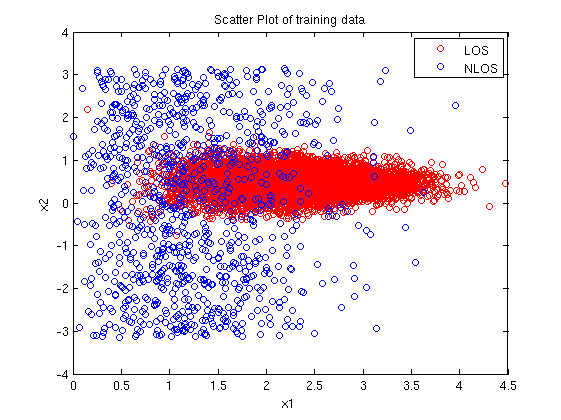
\includegraphics[bb=0 0 449 336]{./figures/5_1_1_trainingdata.png}
 % 5_1_1_trainingdata.png: 561x420 pixel, 90dpi, 15.83x11.85 cm, bb=0 0 449 336
 \caption{Trainingsdatensatz}
 \label{abb:trainingdata}
\end{figure}

\begin{enumerate}
 \item 

\begin{equation}
 p(x_1|t=NLOS) = \frac{x_1}{\sigma^2} exp(\frac{-x^2}{2\sigma^2})
\end{equation}
\begin{equation}
 log(p(x_1^1, ..., x_1^N| \sigma)) = log \prod_{n=1}^N p(x_1^n|NLOS) = \sum_{n=1}^N log(\frac{x_1}{\sigma^2} exp(\frac{-x^2}{2\sigma^2}))
\end{equation}

\begin{equation}
\frac{\partial}{\partial \sigma} = \frac{-2N}{\sigma} + \sigma^{-3} \cdot \sum_{n=1}^N (x_1^n)^2 = 0
\end{equation}
\begin{equation}
 \sigma = \sqrt{\frac{\sum_{n=1}^N (x_1^n)^2}{2N}}
\end{equation}


\item -
\item Die Normalisierung erfolgt durch Multiplizieren jedes Balkens des Histogramms mit dem folgenden Normalisierungsfaktor:
\begin{equation}
 \frac{\#Balken}{(\sum N) * X(end) - X(1)}
\end{equation}
Wobei N die Balkenhöhe und X der zugehörige Balkenmittelpunkt auf der X-Achse darstellt
\item 
ML-Klassifikation: Es wurden 85.1455\% korrekt klassifiziert \\
Bayes-Klassifikation: Es wurden 93.8364\% korrekt klassifiziert \\
Mittels der Bayes Klassifikation lässt sich aufgrund der Priorwahrscheinlichkeit ein besseres Ergebnis erzielen.
Die gute Klassifikationsperformance beruht aber eigentlich nur darauf, dass die meisten Daten LOS sind und nur
wenige NLOS sind. Währe die Priorwahrscheinlichkeit für NLOS und LOS gleich, würde man deutlich schlechtere Ergebnise
erzielen.
\item




\end{enumerate}

\begin{figure}[ht!]
 \centering
 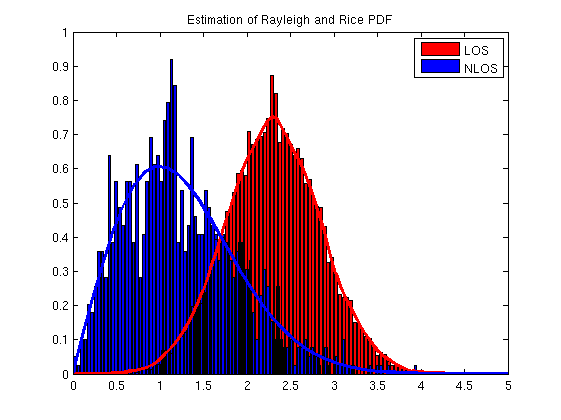
\includegraphics{./figures/5_1_1_estimation.png}
 % 5_1_1_trainingdata.png: 561x420 pixel, 90dpi, 15.83x11.85 cm, bb=0 0 449 336
 \caption{Estimation of PDF-Parameters}
 \label{abb:estimation}
\end{figure}


\begin{figure}[ht!]
 \centering
 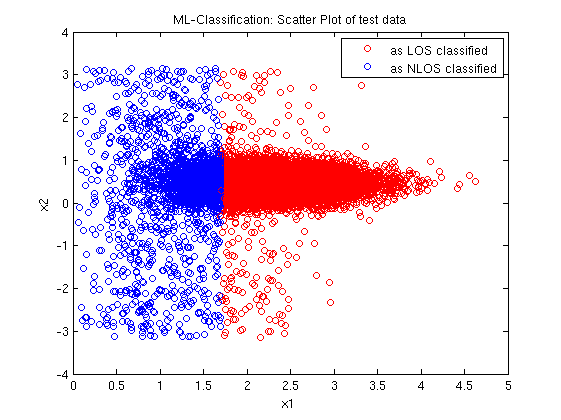
\includegraphics{./figures/5_1_1_ml.png}
 % 5_1_1_trainingdata.png: 561x420 pixel, 90dpi, 15.83x11.85 cm, bb=0 0 449 336
 \caption{ML-Klassifikation}
 \label{abb:ml}
\end{figure}

\begin{figure}[ht!]
 \centering
 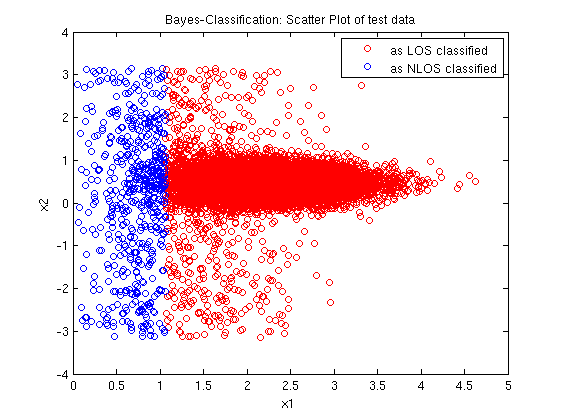
\includegraphics{./figures/5_1_1_bayes.png}
 % 5_1_1_trainingdata.png: 561x420 pixel, 90dpi, 15.83x11.85 cm, bb=0 0 449 336
 \caption{ML-Klassifikation}
 \label{abb:bayes}
\end{figure}

\clearpage

\section{Classification using both amplitude and phase}

Durch die Einführung der Phase ist viel mehr Information verfügbar als durch die Amplitude alleine, was die Performance der Klassifikation deutlich verbessern sollte.

\subsection{Likelihood models}

Schätzen der Normalverteilung der LOS-Phase:

$$ p(x_2 | t = \mathrm{LOS}) = \frac{1}{\sqrt{2 \pi} \sigma_{x_2}} exp(-\frac{(x - \mu_{x_2})^2}{\sigma_{x_2}^2}) $$
$$ \mu_{x_2} = \frac{1}{N_{LOS}} \sum_{x \in LOS} x $$
$$ \sigma_{x_2}^2 = \frac{1}{N_{LOS}} \sum_{x \in LOS} (x - \mu_{x_2})^2 $$

Die Verteilung der NLOS-Phase ist uniform:

$$ p(x_2 | t = \mathrm{NLOS}) = \frac{1}{2 \pi} $$

Abbildung \ref{fig:5_1_2_estimation} zeigt die ermittelten Schätzwerte für die Verteilungen der Phase. Man erkennt, dass die Schätzwerte gut mit den Testdaten übereinstimmen.

\begin{figure}[h!]
  \centering
  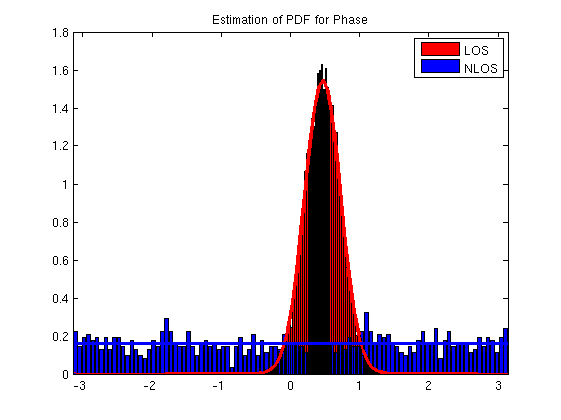
\includegraphics[width=0.75\textwidth]{./figures/5_1_2_estimation.png}
  \caption{Normalisierte Histogramme der geschätzen Verteilungen der Phase}
  \label{fig:5_1_2_estimation}
\end{figure}


\subsection{ML-Klassifikation}

Abbildung \ref{fig:5_1_2_ml} zeigt die Klassifikation mit ML. Durch die zusätzliche Information der Phase können die beiden Bereiche besser unterschieden werden als nur durch die Amplitude. Die Erkennung funktioniert in diesem Beispiel schon recht gut, ein gewisser Bereich (linker Bereich von LOS) wird jedoch noch falsch klassifiziert.

\texttt{blah}

\begin{figure}[h!]
  \centering
  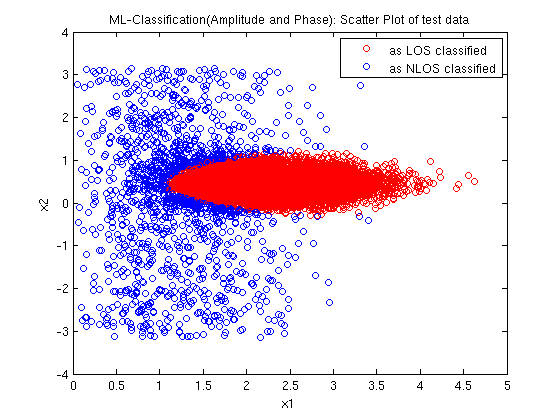
\includegraphics[width=0.75\textwidth]{./figures/5_1_2_ml.png}
  \caption{Klassifikation der Daten durch Most Likelihood Schätzer}
  \label{fig:5_1_2_ml}
\end{figure}


\subsection{Bayes-Klassifikation}

Abbildung \ref{fig:5_1_2_bayes} zeigt die Klassifikation mit Bayes. Wie beim ML-Schätzer ist die Klassifikation besser als ohne Phaseninformation. Die Erkennung funktioniert mit Bayes-Klassifikator noch etwas besser als mit ML, da hier auch der vorher falsch klassifizierte Bereich richtig erkannt wird.

\texttt{blah}

\begin{figure}[h!]
  \centering
  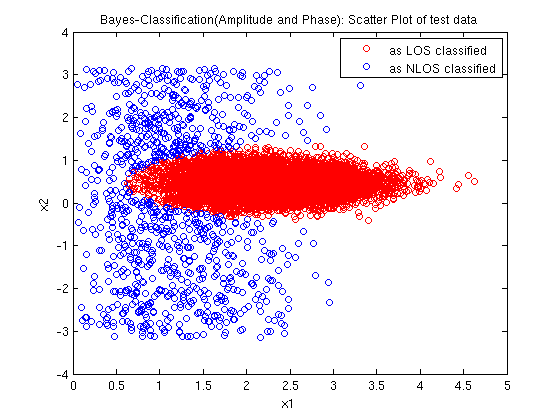
\includegraphics[width=0.75\textwidth]{./figures/5_1_2_bayes.png}
  \caption{Klassifikation der Daten durch Bayes Schätzer}
  \label{fig:5_1_2_bayes}
\end{figure}

\clearpage

\newpage

\chapter{Listings}

%\section{Classification using the amplitude only}
\lstinputlisting[language=matlab]{../implementation/ue5_1.m}
%\section{Classification using both amplitude and phase}
%\lstinputlisting[language=matlab]{../implementation/lda.m}


% **************************************************************************************************
% **************************************************************************************************

%\appendix
%\bibliographystyle{/.base/ieeetran}
%\bibliography{_bibliography}

% place all floats and create label on last page
\FloatBarrier\label{end-of-document}
\end{document}

